\documentclass[a4paper, 12pt]{report}

\usepackage{graphicx}

\begin{document}

% Title
\title{Third assignment documentation}
% Author
\author{Le Minh Nghia - AAOGMU}
\maketitle
\pagenumbering{Roman}
% Table of contents:
\tableofcontents

%CHAPTER:
\chapter{Assignment's description}
\pagenumbering{arabic}
	Yogi Bear wants to collect all the picnic baskets in the forest of the Yellowstone National
Park. This park contains mountains and trees, that are obstacles for Yogi. Besided the
obstacles, there are rangers, who make it harder for Yogi to collect the baskets. Rangers
can move only horizontally or vertically in the park. If a ranger gets too close (one unit
distance) to Yogi, then Yogi loses one life. (It is up to you to define the unit, but it should
be at least that wide, as the sprite of Yogi.) If Yogi still has at least one life from the
original three, then he spawns at the entrance of the park.

	During the adventures of Yogi, the game counts the number of picnic baskets, that Yogi
collected. If all the baskets are collected, then load a new game level, or generate one. If
Yogi loses all his lives, then show a popup messagebox, where the player can type his
name and save it to the database. Create a menu item, which displays a highscore table of
the players for the 10 best scores. Also, create a menu item which restarts the game
%CHAPTER:
\chapter{Usage}

Go to "out/production/YogiBear/" and call cmd, then run "java MainWindow".

%CHAPTER:
\chapter{UML Diagram}
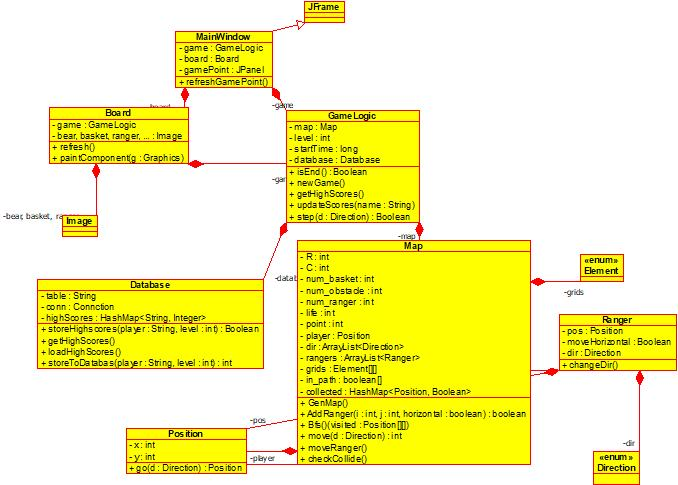
\includegraphics[scale=1.0]{class_diagram.jpeg}

%CHAPTER:
\chapter{Implementation}

\textbf{Generating Level}

Firstly, I generated the number of baskets using random function. After that, I distributed them into the map. Now we need to place rangers and obstacles so that the game is always playable. My approach was using BFS from Yogi starting point (0, 0) to every cell on the map, while traversing, I stored the parent of each cell (in BFS tree) into an 2D matrix. With that, for every basket, I could trace back to the starting point and created a path. Now we could randomly put obstacles into any cell except those are belonged to one of the paths. The hardest part was placing rangers, since they could be anywhere but obstacles, to make sure there is a way to win, we need to put some conditions. The first one was the movement range of a ranger must be $> 2$, because if the range is only 2 then the bear cannot avoid the ranger (The ranger will catch the bear if they are one unit distance). Secondly, in a small area (3x3) there should not exist 2 or more ranger, since it will become impossible to go through. There were also some small corner cases to handle. After putting those conditions, now we can safely generate a map which is solvable and quite random (depend on random generator of Java).

%CHAPTER:
\chapter{Events and event handlers connection}
\begin{description}
	\item[Exit] Will be called when clicked on the close button.
	\item[Player move] when pressed WASD, player will move up, left, down, right.
	\item[Store to database] When the game is end, a box will appear and player can enter their name, after that it will store (player, level) to the database
	\item[Menu Item] When clicked on one of the item in the game menu, a event will happen depends on the item.
\end{description}

\end{document}

